\section{Backend}
Das Backend betreibt unabhängig vom Frontend eine eigene Datenbank und definiert
zusätzlich eigene Methoden, die die volle Kontrolle über diese DB bieten.
Weiterhin definiert das Backend einige Konsolen Kommandos, welche die 
komfortable Nutzung sowie Administration von ctl-Systemen auf Clustern 
sowie Nutzer-PCs ermöglicht.   

\subsection{Datenbankstruktur und ihre Zugriffsmethoden}
  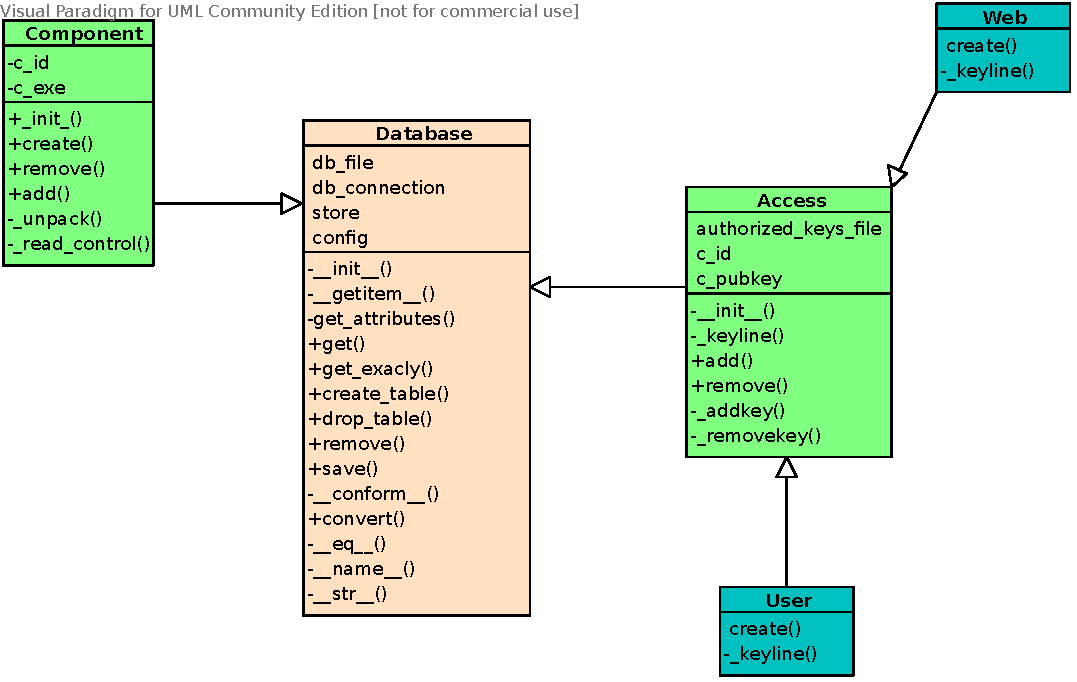
\includegraphics{bilder/clsdiagrambackend.pdf}

Database ist die Vaterklasse. Sie besitzt alle wichtigen Methoden,
die nötig sind, um die Datenbank des Backends zu
betreiben(create(),save(),remove(),get()).

Component stellt die Tabelle \glqq Component\grqq\ in der DB dar und 
spezifiziert deren Attribute \glqq id\grqq\ und \grqq exe\grqq. Component 
erbt von Database, um ihre Tabelle zu modifizieren. Dazu kommen eigene 
Methoden, um Komponenten hochzuladen etc.

Access ist wichtig, um ssh Zugriffmodifikationen zu ermöglichen.
Alle Klassen, die dies möchten, werden von dieser Klasse abgeleitet.
Access erbt zudem von Database.

User und Web erben von Access und damit indirekt auch von Database.
Sie stellen die Tabelle User bzw. Web in der DB dar.

\subsection{

